\subsection{20}
\begin{myfrag}

Beweise dass alle reversiblen Kreisprozesse den gleichen Wirkungsgrad haben
müssen. Wie kann man dies zu einer thermodynamischen Definition der
Temperatur nutzen?
\end{myfrag} \quad \\
Siehe Abbildung 1.1: \\[2ex]
Behauptung: Alle reversiblen Kreisprozesse haben den gleichen Wirkungsgrad.\\[2ex]
Annahme: $\eta' <\eta$ \\[2ex]
$$\eta = \dfrac{|\Delta W|}{|\Delta Q_H |} \quad \eta' = \dfrac{|\Delta W|}{|\Delta Q_H' |}$$ 
$$\eta' < \eta \Rightarrow \dfrac{|\Delta W|}{|\Delta Q_H' |} < \dfrac{|\Delta W|}{|\Delta Q_H |} \\ \Rightarrow | \Delta Q_H'| > | \Delta Q_H | $$
$\Rightarrow $ Wärme wird spontan von kalten zum heißen Reservoir überführt $\nRightarrow$ Zweiter Hauptsatz. \\[2ex]
Wirkungsgrad reversibler Kreisprozesse: \\
$$\eta = 1 - \dfrac{T_K}{T_H} \qquad \dfrac{|\Delta Q_H|}{|\Delta Q_K|} = \dfrac{T_H}{T_K}$$
%TODO ok ist jetzt zweimal drin...
 
\subsection{21}
\begin{myfrag}
Beschreibe den Carnot Kreisprozess und skizziere die dazugehörigen p-V und S-T
Diagramme. Berechne den Wirkungsgrad für reversible Kreisprozesse
\end{myfrag}
\begin{figure}[H]
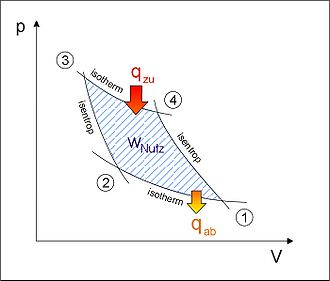
\includegraphics[width=5cm]{Bilder/Frage21pV.jpg} 
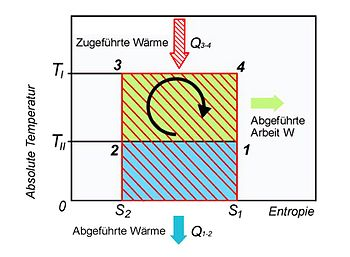
\includegraphics[width=6cm]{Bilder/Frage21TS.jpg} 
\caption{\textbf{Links} P-V Diagramm \textbf{rechts} T-S Diagramm eines Carnot Prozesses}
\end{figure}
Carnot
\begin{enumerate}
\item isotherme Expansion
\item adiabatische Expansion
\item isotherme Kompression
\item adiabatische Kompression
\end{enumerate}
Nach einem Durchgang gilt $ \Delta E = \Delta W + \Delta Q = 0$
\\[2ex]
$\left. \begin{array}{c} \Delta Q_H = \int_1 TdS = T_H(S_b-S_a) > 0 \\ \Delta Q_K = \int_1 TdS = T_K(S_a-S_b) > 0
\end{array} \right\rbrace \Delta W + \Delta Q_H + \Delta Q_K = 0 \ \Rightarrow \ \Delta W = - \Delta Q_H - \Delta Q_K$ \\[1ex]
$\Rightarrow$  Arbeit wird Produziert \\[2ex]

$$\eta = - \dfrac{\Delta W}{ \Delta Q_H}$$ 
$$ = \dfrac{\Delta Q_H + \Delta Q_K}{\Delta Q_H}$$ $$= \dfrac{T_H(S_b-S_a) + T_K(S_a -S_b)}{T_H(S_b-S_a)}$$ 
$$=\dfrac{T_H-T_K)(S_b-S_a)}{T_H(S_b-S_a)}$$ 
$$ = 1 -\dfrac{T_K}{T_H}$$


\subsection{22}
\begin{myfrag}
Beschreibe den Stirling Kreisprozess und skizziere das dazugehörige p-V
Diagramm. Wie könnte man einen realistischen Stirling Motor konstruieren?
Beschreibe eine geeignete Kolbenanordnung und die einzelnen Schritte des
Motors.
\end{myfrag}
\quad \\
\begin{enumerate}
\item isotherme Expansion
\item isochore Wärmeabfuhr
\item isotherme Kompression
\item isochore Wärmezufuhr
\end{enumerate}
$$ W = Q_{zu}-|Q_{ab}|$$
$$Q_{41} = |Q_{23}|$$
Bestehend aus Verdränger- und Arbeitskolben, man braucht Wärmegefäße $\dfrac{\pi}{2} $ Phasenverschoben.
\begin{figure}
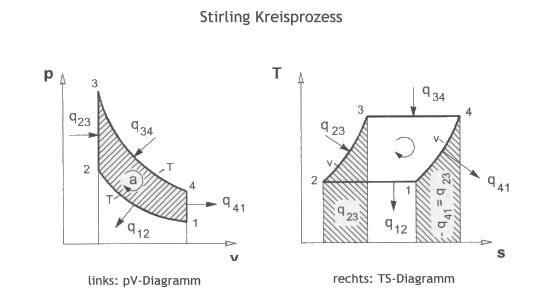
\includegraphics[width=7cm]{Bilder/Frage22pv.jpg} 
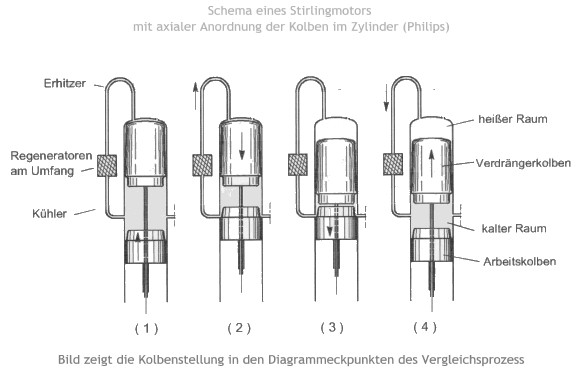
\includegraphics[width=7cm]{Bilder/Frage22Aufbau.jpg} 

\caption{\textbf{Links} P-V Diagramm \textbf{Mitte} T-S Diagramm \textbf{Rechts} Aufbau eines Axialen Stirlingmotors}
\end{figure}
\subsection{23}
\begin{myfrag}
Was sind wichtige Gründe, dass reale Maschinen einen geringeren Wirkungsgrad
haben? Wie kann die Entropieproduktion errechnet werden?
\end{myfrag}
\quad \\
\begin{itemize}


\item Reibung: Arbeit $\Rightarrow$ Wärme \\
Wärme wird bei endlichen Temperatursprüngen Überführt.
\item Regeneratorwirkung ist beschränkt
\item diskontinuierliche Kolbensteuerung
\item Druckverlust
\item Wärmeverlust
\end{itemize}
$$\dfrac{|\Delta Q|}{T_H} < \dfrac{| \Delta Q|}{T_K} \quad \Rightarrow \quad \Delta S_H + \Delta S_K > 0 $$ 
Entropieproduktion durch endliche Temperatursprünge. 
$$ \Delta S = \Delta Q \left( \dfrac{1}{T_K} - \dfrac{1}{T_H}\right) $$
\subsection{24}
\begin{myfrag}
Argumentiere, dass für effiziente Prozesse die Temperaturunterschiede beim
Überführen von Wärme möglichst klein sein sollten.
\end{myfrag}
\quad \\
Entropieproduktion bei endlichen Temperatursprüngen. \\ $$ \Delta S = \Delta Q \left( \dfrac{1}{T_K} - \dfrac{1}{T_H}\right) $$

\chapter{Statistische Mechanik}
\section{Kombinatorik}
\subsection{25}
\begin{myfrag}
\end{myfrag}
\subsection{26}
\begin{myfrag}
\end{myfrag}
\subsection{27}
\begin{myfrag}

\end{myfrag}
\subsection{28}
\begin{myfrag}
Was ist eine Wahrscheinlichkeitsverteilung? Wie werden Erwartungswerte
allgemein berechnet?
\end{myfrag} \quad \\
Jeder Mikrozustand hat eine Wahrscheinlichkeit $P_r$ bzw. $P(\{ \vec{r},\vec{p} _i \} )$ \\ Eine Dichtematrix $\rho = \sum_r P_r \left|r\right\rangle \left\langle r \right| $ ist ein Operator , der die Wahrscheinlichkeitsverteilung beschreibt. $\exists$ Basis $\left| r \right\rangle$ die $\rho $ diagonalsiert, i.A. nicht diagonale Erwartungswerte einer Größe $\Omega $ ist durch \\[1ex]
$<\Omega > = \int \Omega ( \{ \vec{r} _i , \vec{p} _i \}) P_i(\{ \vec{r} _i , \vec{p} _i \} ) d\Gamma $\\[1ex]
$<\Omega> = tr(\rho \Omega )= \sum _ r P_r \left\langle r \right| \Omega \left| r \right\rangle $ \\
Fluktuationen: \\[1ex]
$\Delta \Omega = \sqrt{\Delta \Omega ^2} = \sqrt{\left\langle (\Omega - \left\langle \Omega \right\rangle ) ^2 \right\rangle} = \sqrt{\left\langle \Omega ^2 \right\rangle - 2 \Omega \left\langle \Omega \right\rangle  + \left\langle \Omega \right\rangle ^2} = \sqrt{\left\langle \Omega ^2 \right\rangle - \left\langle \Omega \right\rangle ^2} \\ \Rightarrow \ \left\langle \Omega ^2 \right\rangle \geqslant  \left\langle \Omega \right\rangle ^2 $
\subsection{29}
\begin{myfrag}
Was besagt der zentrale Grenzwertsatz?
\end{myfrag} \quad \\
Der zentrale Grenzwertsatz besagt, dass für $ \Omega = \sum \limits_{i=1}^n y_i $ d.h. eine Summe von sehr vielen Zufallsvariablen $y_i$ mit beliebiger identischer Verteilung $P_y(y_i)$ gilt ( im Grenzwert $ n \rightarrow \infty) $ \\[1ex]
$ P (\Omega ) = \dfrac{1}{\sqrt{2 \pi}\Delta \Omega } \exp\left(- \dfrac{1}{2} \left( \dfrac{\Delta \Omega - \left\langle \Omega \right\rangle ^2}{\Delta \Omega} \right) \right)$  \qquad $ \left\langle \Omega \right\rangle  = \sum \limits_{i=0}^n \left\langle y_i \right\rangle = n \left\langle y \right\rangle $